\chapter{Introducción}
\label{cap:introduccion}
	Durante los últimos años hemos sido testigos del avance y desarrollo de las Tecnologías de la Información y Comunicación (TIC) en zonas urbanas de todo el planeta y en vías y poblaciones rurales  de países desarrollados. Este rápido avance tiene como motores la política pública y la regulación, que allá donde es posible imponen a los operadores obligación de determinados servicios considerados básicos, y la inversión que realizan los operadores de telecomunicación por iniciativa propia para satisfacer la creciente demanda de servicios de comunicaciones allá donde las concentraciones de población fija o en tránsito aseguran un retorno de la inversión.\\
	
	Pese a estos avances que promueven la evolución de la sociedad y su desarrollo a nivel mundial, existen zonas en las cuales dicha evolución apenas se manifiesta. Esta diferencia se conoce como "brecha digital", y se observa sobre todo en países en vías de desarrollo, y más en concreto entre las zonas rurales y urbanas de los mismos, generando desigualdades en la población y en su calidad de vida.\\
	
	Hoy en día, gran parte de la población que ocupa esas zonas rurales, principalmente en países en desarrollo, no tiene acceso a servicios TIC. Esto es debido a que las soluciones y modelos convencionalmente empleados por los operadores no son sostenibles en términos de negocio, ya que su rentabilidad no está garantizada en lugares con baja densidad poblacional, especialmente cuanto más alejados están de los focos de concentración de la población. Además, en estas zonas el poder adquisitivo de la población suele ser bajo o muy bajo, y los relativamente altos costes de los sevicios de telecomunicaciones suponen un esfuerzo económico importante que entra en competencia con los gastos asociados a servicios más básicos como la salud o la educación.\\
	
	Por tanto, el desarrollo de las TIC no sólo implica obtener acceso a los propios servicios de telecomunicaciones, sino que también implica desarrollar y fomentar el resto de sectores sociales y económicos. Para ello, existen medidas y soluciones propuestas de bajo coste que se adaptan a las condiciones de viabilidad de negocio y requisitos de la población, consiguiendo atenuar la "brecha digital" y asegurando una plena integración de estos países en la sociedad de la información.
	

\section{Contexto}
Durante los últimos años, América Latina ha sido testigo de un fuerte desarrollo en la telefonía celular, y a lo largo y ancho del continente es raro el espacio urbano o semi-urbano que no dispone de cobertura 3G o 4G; lo mismo sucede con las vías de comunicación importantes (carreteras principales u otras zonas de tránsito), al menos en los países emergentes. Sin embargo, aún existen amplias zonas rurales que permanecen completamente aisladas de las grandes redes de telecomunicación, en las cuales no existe una sostenibilidad por parte de las grandes operadoras de telecomunicaciones. La razón de esto es la no viabilidad de negocio por parte de las mismas, que no se aseguran la recuperación de la inversión. \\

El caso peruano es paradigmático. El Gobierno ha hecho importantes esfuerzos en los últimos tiempos para llevar infraestructura de fibra óptica a la mayor cantidad posible de poblaciones en todo el territorio nacional, y ha incentivado la extensión privada de infraestructuras rurales mediante iniciativas como la creación legal de la figura del Operador de Infraestructura Móvil Rural (OIMR), cuyo objetivo es ofrecer ventajas competitivas para la interconexión de dichas zonas. Como consecuencia de lo anterior, hay importantes zonas del país sin casi infraestructuras de telecomunicación, destacando en este sentido zonas de sierra en la Cordillera de los Andes, y sobre todo zonas de selva en la Amazonía.\\

Un aumento sustancial de la conectividad en estas áreas más desatendidas tendría impacto en muchos sectores: provocaría una mejora de la atención sanitaria, una modernización del sistema educativo y un impulso para el comercio rural, todo ello de manera eficiente, permitiendo a la población rural y al sistema público un ahorro importante en inversión.\\
	
Con esa interconexión como objetivo final, la Fundación Enlace Hispano Americano de Salud (EHAS), la Universidad Rey Juan Carlos (URJC) y la Universidad Pontificia Católica de Perú (PUCP), junto a otras contrapartes en función de los proyectos concretos, trabajan conjuntamente en el uso apropiado de las TIC, centrándose en el desarollo de sistemas de telecomunicaciones apropiados para los escenarios rurales, y en la creación de servicios destinados a la calidad de vida de la población rural (telemedicina, teleducación, etc).\\
	
En 2013, estas entidades en consorcio con otros socios europeos y latinoamericanos iniciaron el proyecto TUCAN3G, el cual buscaba combinar nuevas tecnologías de acceso celular basadas en femtoceldas 3G con redes de transporte heterogéneas basadas en redes inalámbricas multisalto y en técnicas de ingeniería del tráfico y de optimización. El objetivo era obtener una solución de conectividad rural barata, sostenible, eficiente, autosuficiente y rentable, y que al mismo tiempo no comprometiera la calidad de los servicios del operador.\\
	
El proyecto TUCAN3G mostró unos resultados muy positivos en cuanto a la viabilidad de desarrollo para llevar señal 3G, y la sostenibilidad del modelo de negocio en esas zonas rurales. Por consiguiente, los objetivos próximos se basaban en impulsar la telefonía móvil y continuar con un modelo de negocio sostenible en zonas rurales aisladas, convirtiendo así a la población en un agente activo de su propio desarrollo.    
	
\section{Proyecto Napo}
	En esta sección detallaremos todo lo referente al proyecto Napo, para comprender la relación con el trabajo realizado.
	
	\subsection{Estructura}
	
	El proyecto Napo está basado en la implementación de una red para la comunicación de centros y puestos de salud ubicados a lo largo del río Napo. La red está dividida en dos zonas, una rural y otra urbana; la localización geográfica de los pueblos involucrados en el proyecto se detalla en la siguiente Figura \ref{NetNapo}. Esta red, inicialmente concebida como red de telemedicina, fue inaugurada en su primera versión en 2007, cuando ya fue desplegada a lo largo de la cuenca del río entre la ciudad de Iquitos, capital del Departamento de Loreto, y la población rural de Cabo Pantoja, última población en la rivera del río antes de cruzar la frontera entre Perú y Ecuador. 
	\begin{figure}[H]
		\centering
		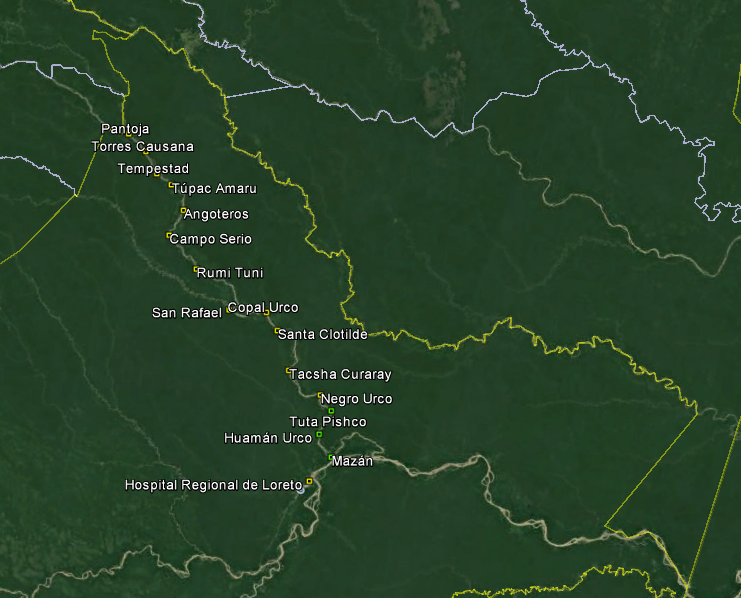
\includegraphics[width=0.7\textwidth]{img/network.png}
		\caption{Localización de la red del Napo.}
		\label{NetNapo}
	\end{figure}
	La zona rural comprende desde Cabo Pantoja (cerca de la frontera ecuatoriana) hasta Huaman Urco. Dentro de esta zona, los pueblos más importantes son Cabo Pantoja y Santa Clotilde, debido a que en ellos existen comodidades y servicios básicos para el trabajo.\\
	Por una parte, la zona urbana está formada por el pueblo de Mazán y la ciudad de Iquitos. Por otra parte, el resto de pueblos que forman la red del Napo son pueblos en los cuales existen limitaciones energéticas y de negocio, por lo que los servicios y prestaciones son precarios.\\\\
	 
	 Posteriormente a su primera etapa como red de telemedicina, operada y mantenida por la Dirección Regional de Salud del Loreto con mucho apoyo de la PUCP, desde 2013 la red fue sometida a una profunda repotenciación y extendida para atender a las necesidades de comunicaciones móviles de la población en general sin dejar de prestar en paralelo los servicios de telemedicina anteriormente citados. La red del Napo está compuesta por la red de transporte (\textit{backhaul}) y la red de acceso. A su vez, la red \textit{backhaul} está formada por enlaces inalámbricos de larga distancia, que utilizan el estándar IEEE 802.11n, desplegados a través de torres ubicadas en los diferentes pueblos que conforman la totalidad de la red. Por otro lado, los servicios de telefonía IP interna, videoconferencia y acesso a Internet,  conforman el total de servicios ofrecidos por la red de telemedicina.\\
	Adicionalmente, la red posee dos accesos satelitales ubicados en Cabo Pantoja y Santa Clotilde, los cuales ofrecen acceso a Internet a toda la red cuando el tráfico no puede salir a través de la ciudad de Iquitos.
	
	\subsection{Utilización de la red}
	En la nueva red del Napo, deben coexistir dos tipos de red de datos, una de ellas destinada a la telemedicina y otra destinada al acceso 3G. Tanto el acceso a Internet de la red de telemedicina, como el de la red 3G será por medio de enlaces satelitales, existiendo dos de ellos para cada una de las redes. Los puntos de acceso satelital para la red de telemedicina estarán ubicados en Cabo Pantoja y Santa Clotilde, mientras que para la red 3G dichas salidas estarán ubicadas en Capo Pantoja y Huaman Urco. En ambas redes se dividirán en grupos las estaciones cliente y se asignarán los accesos satelitales. En caso de indisponibilidad de una pasarela satelital, se reconducirá el tráfico existente por el acceso satelital restante (si éste estuviera disponible).\\
	
	Esta nueva red ha de cumplir con todos los requisitos y necesidades individuales de las redes que la componen y, a su vez, debe ofrecer calidad de servicio. Para la coexión de tráficos se ha planteado una implementación de enrutamiento dinámico, separación de tráfico y política de QoS (Calidad de Servicio); todo ello para conseguir acceso a los servicios ofrecidos por cada red y poder acceder, o redirigir, el tráfico a un gateway determinado. A continuación, describiremos los servicios y requisitos mínimos necesarios para cada una de las redes.\\
	
	Por un lado, la red de telemedicina compuesta por 16 estaciones clientes (centros y puestos de salud), debe ofrecer servicios internos de telefonía IP, videoconferencia y acceso a Internet. Para los servicios de telefonía IP, videoconferencia y acceso a Internet es deseable que todas las estaciones cliente puedan comunicarse de forma simultánea entre sí.\\
		
	Por otro lado, la red 3G estará compuesta por 8 centros, los cuales ofrecerán este servicio. El acceso al \textit{core} 3G de Telefónica del Perú será por medio de dos enlaces satelitales, ubicados en Huaman Urco y Cabo Pantoja.\\
	
	Tras unas primeras pruebas sobre el diseño inicial, recogidas en la Tabla \ref{table:RLPUCP}, vemos como la capacidad de tráfico más restrictiva por enlace es de 44 Mbps; por tanto, se usará este valor como parámetro mínimo en cuanto a capacidad para el resto de radioenlaces. Otra restricción a tener en cuenta es la climatológica, puesto que la red es extensa y existe la posibilidad de que diferentes situaciones degraden la señal.
		
\section{Objetivos del proyecto}
	El objetivo del proyecto Napo es implementar el servicio de acceso de telefonía móvil, provisto de celdas 3G, para que sea compatible con los servicios ya existentes en la red de telemedicina. Para ello, se reemplazarán los equipos de los emplazamientos involucrados en el proyecto. La finalidad de este cambio es mejorar las capacidades de los enlaces radio, para la coexión de tráfico de telefonía celular 3G y los servicios de telemedicina. En orden con lo anterior, para el acceso al \textit{core} 3G de Telefónica del Perú, se desarrollarán dos nuevos accesos satelitales ubicados en Cabo Pantoja y en Huaman Urco.\\
	
	El objetivo de este Trabajo Fin de Grado consiste en asegurar que la solución técnica desarrollada y desplegada por el Proyecto Napo sea técnicamente apropiada y sostenible, y que mantenga los niveles de calidad de servicio necesarios para una red que da soporte a dos redes lógicas independientes: la red 3G de Telefónica y la red de telemedicina pre-existente. Este trabajo se hace en cooperación internacional con el equipo de ingeniería del GTR (Grupo de Telecomunicaciones Rurales) de la PUCP, que son responsables en el proyecto Napo de tomar muchas de las decisiones de diseño. De esta forma, en este trabajo se realizará fundamentalmente una cooperación para la toma de decisiones de diseño, y una auditoría técnica para verificar que dichas decisiones cumplen con las especificaciones previas de la red. Para ello, se realizarán configuraciones equivalentes a las existentes en la nueva red del Napo en laboratorio y se propondrán soluciones respecto a la gestión y monitorización de la red.
	 
\section{Organización del documento}
	La organización correspondiente al Trabajo Fin de Grado viene detallada a continuación.\\
	
	En el primer capítulo, se hace una introducción al desarrollo de las TIC en América latina y, más en concreto, al contexto existente en la cuenca del río Napo. Se presenta la red desplegada en el proyecto TUCAN3G mostrando los resultados obtenidos, y procediendo a su posterior análisis. Por último, se detalla la relación del proyecto Napo con el Trabajo Fin de Grado.\\
	
	En el segundo capítulo, se describirá el estado del arte referente a las diferentes tecnologías y protocolos utilizados en el proyecto. Por un lado, se realizará una descripción de las soluciones propuestas para redes de transporte en zonas rurales. Por otro lado, se introducirá la monitorización y gestión de redes para nuestro trabajo, y se describirán las diferentes soluciones software posibles.\\
	
	En el tercer capítulo, se explicará de manera detallada las principales características de los equipos propuestos como solución, así como una breve introducción al protocolo de pruebas propuesto por la PUCP.\\
	
	En el cuarto capítulo se detallan el protocolo de pruebas utilizado con el objeto de conocer que equipo encaja dentro del marco del proyecto como solución. De igual forma, se hará una descripción detallada de la configuración y diseño realizado a nivel de laboratorio para llevar a cabo la realización de pruebas.\\
	
	En el quinto capítulo, se procede a analizar y contrastar los resultado obtenidos. Dichos resultados deberán aportar una solución en cuanto a los requisitos de diseño de la nueva red del Napo y detectar anomalías si las hubiera.\\
	
	En el sexto capítulo, se muestran las conclusiones y competencias adquiridas a partir de este Trabajo Fin de Grado, y una visión acerca de futuros trabajos basados en este proyecto.\\
	
	En el séptimo capítulo, se muestran las tablas y código utilizado para el desarrollo de este Trabajo Fin de Grado.\\
	
	Finalmente, se encuentra la bibliografía utilizada para llevar a cabo este Trabajo Fin de Grado.